%%%%%%%%%%%%%%%%%%%%%%%%%%%%%%%%%%%%%%%%%%%%%%%%%%%%%%%%%%%%%%%%%%
%%%%%%%% ICML 2014 EXAMPLE LATEX SUBMISSION FILE %%%%%%%%%%%%%%%%%
%%%%%%%%%%%%%%%%%%%%%%%%%%%%%%%%%%%%%%%%%%%%%%%%%%%%%%%%%%%%%%%%%%
\documentclass{article}
\usepackage{times}
\usepackage{graphicx} % more modern
\usepackage{subfigure} 
% For citations
\usepackage{natbib}
% For algorithms
\usepackage{algorithm}
\usepackage{algorithmic}

% Stuff that I added in (Daniel Seita) 
\usepackage{amsmath,amssymb,amsthm,enumitem,verbatim,url}
\graphicspath{ {Images/} }
\newtheorem{thm}{Theorem}[section]
\newtheorem{conj}[thm]{Conjecture}
\newtheorem{cor}[thm]{Corollary}
\newtheorem{lem}[thm]{Lemma}
\newtheorem{prop}[thm]{Proposition}
\newtheorem{exa}[thm]{Example}
\newtheorem{defi}[thm]{Definition}
\newtheorem{exe}[thm]{Exercise}
\newtheorem{rek}[thm]{Remark}
\newtheorem{que}[thm]{Question}
\newtheorem{prob}[thm]{Problem}
\newtheorem{cla}[thm]{Claim}
% End of stuff I added in

% As of 2011, we use the hyperref package to produce hyperlinks in the resulting PDF.  If this breaks your system, please commend out the following
% usepackage line and replace \usepackage{icml2014} with \usepackage[nohyperref]{icml2014} above.
\usepackage{hyperref}

% Packages hyperref and algorithmic misbehave sometimes.  We can fix this with the following command.
\newcommand{\theHalgorithm}{\arabic{algorithm}}

% Employ the following version of the ``usepackage'' statement for submitting the draft version of the paper for review.  This will set the note in
% the first column to ``Under review.  Do not distribute.''
%\usepackage{icml2014} 
% Employ this version of the ``usepackage'' statement after the paper has been accepted, when creating the final version.  This will set the note in
% the first column to ``Proceedings of the...''
\usepackage[accepted]{icml2014}

% The \icmltitle you define below is probably too long as a header.  Therefore, a short form for the running title is supplied here:
\icmltitlerunning{The Distributed Retired Traveling Salesman Problem}

\begin{document} 

\twocolumn[
\icmltitle{The Distributed Retired Traveling Salesman Problem}

% It is OKAY to include author information, even for blind submissions: the style file will automatically remove it for you unless you've provided the
% [accepted] option to the icml2014 package.
\icmlauthor{Daniel Seita}{dts1@williams.edu}
\icmlauthor{Ziang Zhang}{zz2@williams.edu}
\icmladdress{Department of Computer Science, Williams College, Williamstown, MA 01267 USA}

% You may provide any keywords that you find helpful for describing your paper; these are used to populate the "keywords" metadata in the PDF but will
% not be shown in the document
\icmlkeywords{distributed systems}

\vskip 0.3in
]

\begin{abstract} 
The use of major online travel agencies has made scheduling long-term travel much easier by allowing users to easily identify a set of flights in just
a few clicks. Current travel agencies allow users to plan out long-term trips involving flights to more than two cities, but they require specific
arrival and departure dates for each city and a city ordering. We present a system that does not burden the user with these decisions. Specifically,
our code takes in two required inputs: a list of cities the user wishes to travel to, and a date range over which they are willing to travel, and
outputs the cheapest set of flights within that range that form a valid route. It essentially solves a harder version of the Traveling Salesman
Problem since costs are not constant between two cities. Under several weak assumptions, and assuming that the number of cities and days is
sufficiently limited, then our algorithm should successfully find the cheapest cost flight in a reasonable amount of time. We present the theoretical
and systematic components of the project and discuss empirical results.
\end{abstract} 

\section{Introduction and Motivation}\label{sec:intro}

The use of major online travel agencies, such as Travelocity\footnote{\url{www.travelocity.com}} and Kayak\footnote{\url{www.kayak.com}}, has made
scheduling long-term travel much easier by allowing users to easily select a set of flights to purchase tickets from. People use a combination of
factors to help them make their decision, such as the total price of the flights and the days they wish to land and depart from a city. Current travel
agencies allow users to plan out trips involving airlines to multiple destinations (see Figure~\ref{fig:travelocity} for an example using
Travelocity), but they require (1) specific dates for each city and (2) an ordering.

This limitation can make searching for flight routes time-consuming for users who are not restricted to arriving at cities on particular dates. For
instance, suppose one resides in New York City (NYC) and wants to schedule a summer trip to Paris, London, and Tokyo from June 1 to June 20, and it
does not matter to him how long he stays in a city. Suppose that it also does not matter the ordering that he arrives at the cities. Thus (for now) we
will only care about the following factors\footnote{For brevity, we list a high-level overview of the problem without getting into too many technical
details; Section~\ref{sec:limitations} describes some of our assumptions and limitations.}:

\begin{itemize}[noitemsep]
    \item The full flight route occurs within the date range (in this case, between June 1 and June 20).
    \item The flight route must arrive and leave at least once for NYC, Paris, London, and Tokyo.
    \item The flight route is valid and logically consistent. For instance, if the first flight takes him from NYC to Tokyo, the second flight in the
    route should not depart from a place other than Tokyo.
\end{itemize}

There are a vast pool of valid flight routes. We might assume that out of all these, one would want the \emph{cheapest} route. Of course, this glosses
over how the user may want to spend some number of days at each city, but this is the most general case.

Unfortunately, finding the cheapest route possible is challenging using current agencies, because they require knowing the arrival and departure dates
for each city. The reason for this is simple: the problem of finding this flight route is a hard problem to solve. In fact, this problem is very
similar to the well-known Traveling Salesman Problem~\cite{Applegate:2007:TSP:1374811}, which asks if there exists a cycle in a graph that touches
each node exactly once (i.e., a Hamiltonian cycle). Each edge has a cost associated with it, and the decision version of the problem, which asks if
there exists a valid Hamiltonian cycle with cost bounded by $B$, is NP-complete~\cite{Kar72}. In our case, we do not force the user to visit each
city exactly once because the cheapest flight through a sequence of cities \emph{may require} visiting a city more than once.

What makes our problem (likely) much harder than the Traveling Salesman Problem is that the cost of an edge between two nodes (i.e., two cities) is
not constant, because flight prices frequently change. We coin our problem the ``Distributed Retired Traveling Salesman Problem.'' ``Retired'' comes
from how we assume that whoever is planning this trip is retired, because otherwise, how would he or she have the time and money?  ``Distributed''
comes from how we incorporate concepts from the design and practice of distributed systems to build software that can tackle this problem. We discuss
the mathematical and systems portions of our solution in Sections~\ref{sec:math} and~\ref{sec:systems}, respectively.

\begin{figure}[t]
\vskip 0.2in
\begin{center}
\centerline{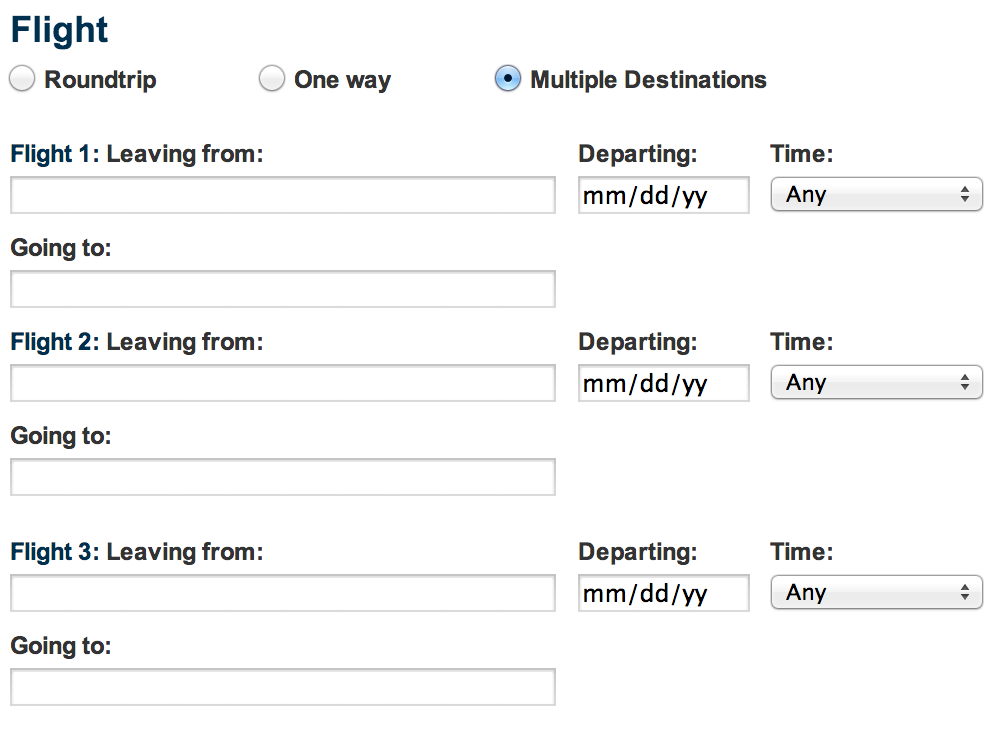
\includegraphics[width=\columnwidth]{travelocity}}
\caption{Travelocity lets users select multiple destinations.}
\label{fig:travelocity}
\end{center}
\vskip -0.2in
\end{figure}

\section{Related Work}\label{sec:related_work}

The Traveling Salesman Problem (TSP) is one of the oldest and most well-known problems in combinatorial optimization. While no exact, polynomial time
solution for the decision problem is known, there is a $3/2$-approximation algorithm due to Christofides~\cite{Chr76}. That algorithm was long the
standard approximation algorithm until a stunning recent result in~\cite{conf/focs/GharanSS11}, which has thus spurred a cascade of additional
research relating to the TSP (e.g.,~\cite{Moemke:2011:AGT:2082752.2082898}).

In contrast to the attention devoted to TSP, there appears to be very little research focusing on the special case of our problem, which introduces
additional challenges. These can be mathematically-oriented, such as how to manage the variable costs, or systems-oriented, such as how to even obtain
the actual flight costs. We have found nothing in the literature that particularly fits our problem.

\section{Mathematical Component}\label{sec:math}

The mathematical portion of our work uses a technique known as \emph{binary integer linear programming}, which falls under the broader category of
optimization techniques. The goal in optimization is straightforward: given a set of variables and a set of constraints, the goal is to find the best,
feasible solution according to some criteria, such as cost (in which case, ``best'' means ``minimal'').

\subsection{Linear and Integer Programming}\label{sec:lin_int_programming}

One of the most commonly-used optimization techniques is linear programming, introduced by Dantzig in~\cite{GVK180926950}.

\begin{defi}\label{defi:linear_programming}
A \emph{linear programming problem} consists of three components: 
\begin{enumerate}[noitemsep]
    \item a finite collection of linear inequalities or equations in a finite number of unknowns, $x_1, \ldots, x_n$;
    \item sign constraints $x_i \ge 0$ on some (possibly empty) subset of the unknowns;
    \item a linear function to be minimized or maximized.
\end{enumerate}
An assignment to the variables $x_1, \ldots, x_n$ satisfying the first two conditions is a \emph{feasible} solution. If it also satisfies the third,
then it is an \emph{optimal} solution~\cite{opac-b1105716}.
\end{defi}

Linear programming has tremendous applications, and a full list of them would be impossible to create. Some problems well-suited to linear programming
include investment management, scheduling problems, and the diet problem. (The last problem concerns the rather interesting question of what is the
minimum cost of a nutritionally adequate diet.) The reason for linear programming's great versatility is the ease at which constraints can be added to
a model.

More specific cases of linear programming are integer and binary linear programming. (Sometimes we drop the ``linear'' part for brevity.)

\begin{defi}\label{defi:integer_programming}
An \emph{integer programming problem} is a linear programming problem with the added restriction that all variables (i.e., unknowns) $x_1, \ldots,
x_n$ are integers.
\end{defi}

\begin{defi}\label{defi:binary_programming}
A \emph{binary integer programming problem} is an integer programming problem with the added restriction that all variables $x_1, \ldots,
x_n$ are such that $x_i \in \{0,1\}$.
\end{defi}

We see that our problem is particularly suited to binary integer programming, because all the possible flights we could take can be viewed as a set of
binary random variables, each of which has value 1 if we decide to take that flight, and 0 otherwise. We now formulate this problem in more detail.

\subsection{An Integer Programming Formulation}\label{sec:int_prog_form}

To start formulating the problem, we make it concrete what we mean by cities, days, and costs.

\begin{itemize}[noitemsep]
    \item We have $n$ cities to reach; we index cities by $i$ or $j$, where $i, j \in \{1, 2, \ldots, n\}$.
    \item We have $t$ consecutive days when we can travel: $t \in \{1, 2, \ldots, m\}$.
    \item The minimum cost for traveling from city $i$ to $j$ on day $t$ is $c_{ijt}$.
\end{itemize}

Using the above lets us define the following variables:

\[
x_{ijt} = \begin{cases}
1 &\mbox{if we go from cities } i \mbox{ to } j \mbox{ on day } t, \\ 
0 & \mbox{otherwise}.
\end{cases}
\]

Thus, a solution to our problem will be the full assignment to each of the above variables. The set of the binary variables that equal one will
(assuming the set has cardinality $k$) correspond to $k$ flights $f_1, \ldots, f_k$ ordered by date.

For now, we make several simplifying assumptions, and defer a more detailed discussion about the realism of this project in
Section~\ref{sec:limitations}. Perhaps the most important one is that we assume each flight is assigned to exactly one day. We also force a valid
solution to have flights on unique days. This means we do not consider issues related to (1) overnight flights (we will pretend they do not exist),
(2) multiple-stop flights on the same day, and (3) possible logistic impossibilities such as flight $f_i$ arriving at 11:59 PM and then the next
flight $f_{i+1}$ departing from the same airport two minutes later (but on the next day).

The goal is to solve this minimization problem:

\begin{equation}
\mbox{Minimize } \sum_{t=1}^{m} \sum_{i=1}^{n} \sum_{j=1}^{n} c_{ijt}x_{ijt},
\end{equation}

\emph{subject to} the following constraints:
\begin{align}
\sum_{i=1}^{n} \sum_{j=1}^{n} x_{ijt} &\le 1 \mbox{ for all } t \in \{1, 2, \ldots, m\}, \\ 
\sum_{t=1}^{m} \sum_{i=1}^{n} x_{ijt} &\ge 1 \mbox{ for all } j \in \{1, 2, \ldots, n\}, \\
\sum_{t=1}^{m} \sum_{j=1}^{n} x_{ijt} &\ge 1 \mbox{ for all } i \in \{1, 2, \ldots, n\}.
\end{align}

The first constraint ensures that we have at most one flight per day, which is generally too restrictive for real-life, but will suffice for now. The
second constraint ensures we enter each city at least once. The third constraint ensures we leave each city at least once. These last two reinforce
the notion that going through the cheapest route may mean visiting several cities more than once.

Sadly, these previous constraints are \emph{not} enough to solve our problem. If we were to use them, we could get a logically inconsistent flight
route due to two main reasons.

\subsubsection{Disjoint Cycles}\label{sec:disjoint_cycles}

The first problem is that the constraints do not prevent disjoint cycles. Figure~\ref{fig:bad_solution} shows a graph with six nodes, which may
represent six cities, and a possible edge assignment that is indicative of the route we take to visit all cities. Assuming the flights are all on
different days, the route satisfies our constraints, because we enter and exit each city at least once, but this is not a Hamiltonian cycle.

\begin{figure}[t]
\vskip 0.2in
\begin{center}
\centerline{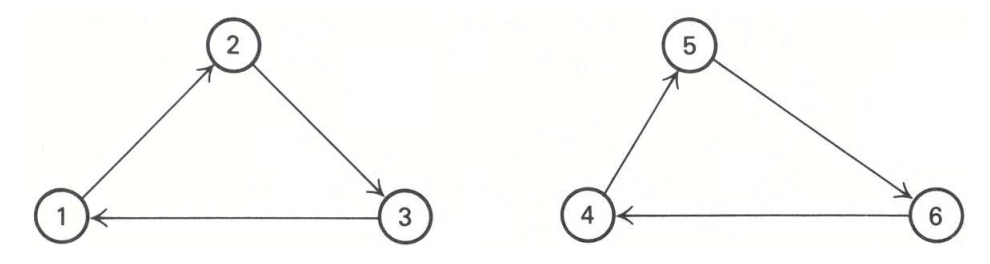
\includegraphics[width=\columnwidth]{bad_solution}}
\caption{This represents two sets of disjoint cycles.}
\label{fig:bad_solution}
\end{center}
\vskip -0.2in
\end{figure}

To prevent disjoint cycles, we need to add constraints that correspond to all the ways we can subdivide the cities into two groups so that both
contain at least two cities. (A subdivision where one group only has one city is already covered by our earlier constraints since we would have to
leave and enter that city at least once, which requires connecting with the other group.) For instance, with the six-variable situation in
Figure~\ref{fig:bad_solution}, one constraint would be
\begin{align}
\sum_{t=1}^{m} (&x_{14t} + x_{15t} + x_{16t} + x_{24t} + x_{25t} + \\
& x_{26t} + x_{34t} + x_{35t} + x_{36t}) \ge 1, \nonumber
\end{align}

which ensures that at least one leg of the tour connects cities 1, 2, and 3 with cities 4, 5, and 6, so this corresponds to the subdivision of
$\{[1,2,3],[4,5,6]\}$. We can characterize the number of constraints we need to add to prevent disjoint cycles.

\begin{lem}\label{lem:cycle_constraints}
In a problem that has $n \ge 4$ constraints, the number of ways to subdivide the cities so that each has two groups is ${n \choose 2} + {n \choose 3}
+ \cdots + {n \choose n-2}$.
\end{lem}

The reasoning is straightforward: we have two groups, and we want to pick the number of elements for one group. We can pick some number out of $n$
elements to be in one group, and assign all the rest to the others.

One technical note is that the number of constraints from Lemma~\ref{lem:cycle_constraints} can be halved by symmetry. Still, the number of equations
needed grows rapidly with respect to $n$, and the need to implement these is why integer programming is a hard task. Integer programming is, in fact,
an NP-hard problem, and the binary case is NP-complete~\cite{Kar72}. In contrast, faster algorithms such as the Simplex method\footnote{The Simplex
Method performs well in practice but its runtime has historically been difficult to evaluate, as in the worst case it \emph{can} run in exponential
time~\cite{Klee1972}. The simplex algorithm has \emph{smoothed complexity} polynomial in the input size; for details about this,
see~\cite{Spielman:2004:SAA:990308.990310}.} are used to solve linear programming problems. Note that simply taking a solution to the linear
programming problem and then rounding it to form a ``solution'' to the integer problem will not work, as we show in Appendix~\ref{app:lin_vs_int}.

\subsubsection{Consecutive Flights in Different Cities}

The second problem with the constraints in Section~\ref{sec:int_prog_form}, which the constraints in~\ref{sec:disjoint_cycles} do \emph{not} resolve,
is that we can get flight orderings that are logically inconsistent in the sense that consecutive flights may not agree in their choice of cities. It
makes no sense, for instance, to have flights $f_i$ and $f_{i+1}$ where $f_i$ takes the participant from NYC to Tokyo, and $f_{i+1}$ takes him or her
from Paris to London.

Unfortunately, fixing the flight ordering by adding in constraints is challenging and requires a large number of equations. Our implementation only
adds in one layer of constraints for here, and defers a complete flight logic check to the code that actually generates the tree. Specifically, for
all pairs of days $t$ and cities $c$ such that $t \in \{1,2,\ldots, m-1\}$ and $c \in \{1,2,\ldots,n\}$ we add in the following constraints:
\begin{align}
\underbrace{\left(\sum_{i\ne c} x_{ict} \right)}_{\text{Term 1}} + \underbrace{\left( \sum_{j\ne c}\sum_{k\ne j} x_{jkt^+}\right)}_{\text{Term 2}} \le 1,
\end{align}
% TODO I think it still works for n+1 days but let me think about it and put stuff in the appendix.

where $t^+$ is shorthand for $t+1$ (which explains why we don't set $t$ to be $m$). Term 1 represents entering city $c$, and Term 2 represents leaving
any city other than $c$. Notice that by our previous constraints, both Term 1 and Term 2 are already bounded by one, so if both are one, then this
indicates that two flights on back-to-back days are not logically consistent. We therefore have the following lemma.

\begin{lem}\label{lem:correctness}
Assuming that we have $n$ cities and $n$ or $n+1$ days as input, solving the binary integer programming problem using the previous constraints will return a
valid, logically consistent solution.
\end{lem}

The correctness of $n$ days in the flight schedule will force correctness in the case of $n+1$ days, but beyond that it is possible to get a logically
invalid flight scheduling. We resolve that issue by not using constraints at all. We just run the problem and, each time a candidate solution is
proposed, check its complete vector for logical consistency.  Thus, it is a ``last-minute'' check that must be passed before a complete assignment to
the variables is accepted.

\subsection{Using Balas' Additive Algorithm}\label{sec:balas}

To actually solve the binary integer programming problem, we use Balas' Additive Algorithm~\cite{doi:10.1287/opre.13.4.517}. This is a special case of
the larger class of branch-and-bound algorithms, which are used to solve integer programming problems. Branch-and-bound algorithms consist of a
systematic enumeration of all candidate solutions, where large subsets of fruitless candidates are discarded by using upper and lower estimated bounds
of the quantity being optimized~\cite{Clausen1997}.

Balas' algorithm makes use of the special properties of binary integer programming problems. Assuming that the costs are all non-negative, and that
variables are indexed according to cost, we want to (1) set all variables to zero in order to minimize total cost, and (2) if we cannot set all
variables to zero due to constraints, then we wish to set the variable with smallest index to one. What results is a rooted tree where each path of
$n$ nodes from the root indicates an assignment to the first $n$ variables. One can use a standard depth-first search to implement the algorithm.  For
brevity we elide additional technical details of the algorithm and refer the reader to Appendix~\ref{app:balas}.




% The second major part of the implementation
\section{Systems Component}\label{sec:systems}

\begin{figure}[t]
\vskip 0.2in
\begin{center}
\centerline{
\includegraphics[width=\columnwidth]{servers}}
\caption{This is our ideal machine setup.}
\label{fig:machines}
\end{center}
\vskip -0.2in
\end{figure}

We now step back from the mathematics and discuss the implementation. Our code that solves the Distributed Retired Traveling Salesman Problem is
made up of several components that form a multi-tiered client-server model (for an introduction to the client-server model,
see~\cite{Tanenbaum:2006:DSP:1202502}). Figure~\ref{fig:machines} gives a rough sketch of our ideal machine setup. We have a front-end server, a
master server, and a group of slave (``crawler'') servers.  

\subsection{Front-end Server}\label{sec:front_end_server}

The front-end server acts as a point of communication between the client\footnote{Somewhat impolitely, we refer to the set of clients, minus Daniel
Seita, as the ``ignorant masses.''} and our master server. It is a Python script that starts on the command line and outputs messages to the client
to let him or her know how to use our system. The front-end serve receives user input, forwards the request to the master server (step \texttt{1} in
Figure~\ref{fig:machines}), listens to the master for the result (step \texttt{6}), and displays it back when ready. Currently, the result is just the
single best list of the flights ordered by departure date. If there is more than one optimal solution, it only returns one of them.

\begin{figure}[t]
\vskip 0.2in
\begin{center}
\centerline{\includegraphics[width=\columnwidth]{front_end_server3}}
\caption{This shows our front-end server.}
\label{fig:front_end_server}
\end{center}
\vskip -0.2in
\end{figure}

Figure~\ref{fig:front_end_server} shows our current front-end server. Here, the hypothetical user made a request to find the cheapest flight route
that touches Atlanta, Chicago, and Los Angeles in the three day period of June 1 through June 3.  Our code ran and returned the (valid) flight route
of Chicago to Los Angeles to Atlanta that costs \$585.

Notice that the front-end server has an optional argument where the user can indicate the minimum number of days between two consecutive flights. (The
example from Figure~\ref{fig:front_end_server} just happened not to use it.) It is straightforward to add more of these optional arguments. If time
permits, we also plan to transform the command-line interface to a website, which will expand our audience of potential clients.


\subsection{Master Server}\label{sec:master_server}

The master server is the workhorse of our system. It takes in the user request sent in from the front-end server from
Section~\ref{sec:front_end_server}. When a request comes in, the master server runs a variety of checks to ensure the user's input is acceptable.  For
instance, given the optional argument where the user can specify the minimum number of days between flights, the server checks that the full date
range is large enough to allow that case to happen. We do not catch all possible cases of pathological inputs, in part because we trust our users not
to wreck the system. (It is interesting to debate about the impact of trust in systems; for now, we gloss over these and refer the reader to sources
such as~\cite{Blaze:2001:RTM:380171.380186}.)
% TODO We can put an appendix in to describe our checks, but I'm getting tired of writing already.

After parsing the input, the master server has two important tasks. The first is that it needs to obtain the cheapest flight that goes from cities $i$
to $j$ on day $t$ for all $n(n-1)m$ possible combinations. It accomplishes this by calling any idle slave servers to look up a single price, which
spawns a new thread. Thus, with $k$ total flights and $\ell$ slaves, we expect each to contribute $k/\ell$ flight prices to the master. This is shown
in Figure~\ref{fig:machines} as \texttt{2} and \texttt{4}. (That we only have two calls to each slave is just for simplicity, since there can be an
arbitrary amount of them.)

Once the master server has all the prices for the flights, it combines this information with the rest of the user request into inputs suitable for
binary integer programming. Computing the cost vector is easy; the challenging part is making sure that the constraints are well-defined. Once the
master sever has determined the constraint matrix, it calls the binary integer programming solver. As discussed in Section~\ref{sec:balas}, this runs
Balas' Additive Algorithm to create the final vector of variable assignments. There, if $x_{ijt} = 1$, then the cheapest valid route involves that
corresponding flight (and 0 otherwise). It is theoretically possible to distribute Balas' algorithm, but for ease of implementation, we currently run
it on one machine, so it is essentially part of the master server. Upon completion, the master server feeds the result back to the client server.

% TODO This old description is not really correct.
% The Master server is the brain of the system. It listens to the user request sent from the front-end server (step \texttt{1} in
% Figure~\ref{fig:machines}). When a request comes in, it first comes up with a list of flight prices on all possible dates and for all possible
% destinations in the problem that we need to get for the computation, distributes the flight price queries among all the slaves (step \texttt{2}),
% gathers all the price data back from the slaves (step \texttt{3}), and combines them. It then upload the combined data to a distributed file system to
% make the data available for parallel computing on all the slaves. Then it starts the parallel computing for the cheapest route using a distributed
% zero-one linear programming algorithm on all slaves (steps \texttt{4} and \texttt{5}). After the computation, it sends the results of the cheapest
% route back to the front-end server (step \texttt{6}).

\subsection{Slave Servers}\label{sec:slave_server}

The slave servers come from our own machines. Originally, we wanted to use PlanetLab~\cite{conf/osdi/PetersonBFM06}, which is a global platform for
deploying and evaluating network services, but it was too complicated to work with. Currently, our system can have an unbounded amount of slave
servers, each of which must be started before the user sends a request. The slave server's purpose is to, upon request from the master server, use a
web crawler to obtain prices of real airlines and relay it back (steps \texttt{3} and \texttt{5} in Figure~\ref{fig:machines}, though again, the
number is arbitrary).

To look up the prices, we implemented a web crawler that extracts prices from the Matrix Airfare Search\footnote{\url{http://matrix.itasoftware.com/}}
database, which is powered by ITA Software and is the best flight database currently available. This induces a natural delay in searching for flights
because the website must be loaded each time for a search, so for small inputs, the flight lookup process is typically much slower than Balas'
algorithm

% TODO This is not really correct.
% We have a group of slave servers that listens to the command of the master server and does the distributed tasks of flight price querying (using the
% web crawler we write) and parallel zero-one linear programming. We will use the Matrix Airfare Search\footnote{\url{http://matrix.itasoftware.com/}}
% database to obtain information about our flights; the information itself will be extracted with our own web crawler. We coin this ``The Retired
% Traveler Problem,'' primarily because if we assume the dates are set far enough apart, it would interfere with a non-retired person's occupation. For
% details on the real problem, see sources such as.


\section{Experiments and Results}\label{sec:experiments_results}

We present a brief experimental analysis of our system. Due to space constraints, we only offer high-level descriptions here and defer complete
results to Appendices.

\subsection{Single-Node Experiments}\label{sec:single_experiment}

We experiment with a variety of inputs on a single node, which means we only use one slave server. Table~\ref{tab:single-node} shows our results on
twenty inputs. The inputs have \texttt{C}s, \texttt{D}s, and \texttt{G}s, denoting the number of cities, days, and gap days between flights (if any).
The main concern is the runtime of our whole system. The ``F Time'' and ``B Time'' columns represent the time (minutes:seconds) to run the flight
checker and Balas' algorithm, respectively. ``V'' represents the set of variables, and the ``Nodes'' column is how many nodes Balas' algorithm
expanded. These values \emph{must be substantially smaller} than the full list of $2^{|V|}$ possible vector assignments. A more complete treatment of
these experiments is in Appendix~\ref{app:single_machine_experiment}.

\begin{table}[t]
\caption{Statistics of our single-crawler system.}
\label{tab:single-node}
\vskip 0.15in
\begin{center}
\begin{small}
\begin{sc}
\begin{tabular}{lcccc}
\hline
\abovespace\belowspace
Input & $|V|$ & F Time & Nodes & B Time \\
\hline
\abovespace
3C 3D    & 18  & 02:31 & 174     & 0:00  \\
3C 4D    & 24  & 04:01 & 717     & 0:00  \\
3C 5D    & 30  & 04:23 & 2845    & 0:00  \\
3C 6D    & 36  & 05:14 & 10336   & 0:00  \\
3C 7D    & 42  & 06:03 & 35902   & 0:00  \\
3C 8D    & 48  & 06:47 & 127570  & 0:01  \\
3C 9D    & 54  & 07:36 & 460872  & 0:08  \\
3C 10D   & 60  & 08:45 & 1472853 & 0:32  \\
3C 11D   & 66  & 09:22 & 4609309 & 2:23  \\
3C 5D 1G & 30  & 04:23 & 2855    & 0:00  \\
3C 6D 1G & 36  & 05:29 & 10136   & 0:00  \\
3C 7D 1G & 42  & 06:07 & 38613   & 0:00  \\
3C 8D 1G & 48  & 06:41 & 125988  & 0:01  \\
3C 9D 1G & 54  & 07:38 & 442564  & 0:08  \\
3C 7D 2G & 42  & 06:23 & 38217   & 0:00  \\
3C 8D 2G & 48  & 06:53 & 125267  & 0:01  \\
3C 9D 2G & 54  & 07:53 & 442122  & 0:08  \\
3C 9D 3G & 54  & 07:48 & 442412  & 0:09  \\
4C 7D    & 84  & 12:21 & 1548120 & 0:45  \\
\belowspace
5C 5D    & 100 & 14:14 & 261089  & 0:10  \\
\hline
\end{tabular}
\end{sc}
\end{small}
\end{center}
\vskip -0.1in
\end{table}

From the results, we see that flight time increases linearly and that Balas' algorithm increases exponentially (as expected). We tried running a three
city, twelve day example, but Balas' algorithm continued for over three hours without getting anything done. It seems like once we start increasing
the number of days and cities beyond what are shown in Table~\ref{tab:single-node}, Balas' algorithm will be the limiting factor of our algorithm.

\subsection{Multi-Node Experiments}\label{sec:distributed_experiment}

The goal now is to understand the impact of 


\section{Limitations}\label{sec:limitations}
% TODO We can cut out some of the limitations here because it's fairly long...

This section addresses a number of issues briefly touched upon in Section~\ref{sec:int_prog_form} and other areas of this paper. We avoid discussing
anything that can be easily added as an extension (e.g., forcing us to start at one particular city, or making the flight route to make a stop at a
city three times).

\subsection{Practical Usage}

One important question to consider is whether our system is practical for real-life use. Our experiments in Section~\ref{sec:experiments_results} show
that it is doable for a small enough input. Ideally, the number of cities would be limited by four, maybe five (which seems reasonable for a trip),
and the number of days bounded based on the number of cities. One of the key limiting factors in our algorithm is the length of the variable vector,
or the number of flights we must consider. In particular, if the user requests a flight route involving $n$ cities over $t$ days, then the total
number of days and flight combinations possible is $n(n-1)t$, which comes from picking one of $n$ cities to start from, one of the $n-1$ remaining
cities to land to, and one of the $t$ days for this flight to occur. This is why the bound on the days should be considered in context with the number
of cities; the fewer cities we have, the more days we can allow.

Our experience shows that if $n(n-1)t$ is bounded by 100, then the problem is generally doable (i.e., completes within a few hours).
A bound of 100 is still prohibitive for an extensive travel trip. If someone wants to travel for a month's worth of days, say $t = 30$, then the
minimum number of flights possible for our system would be $3\cdot 2\cdot 30 = 180$, already quite prohibitive. The situation gets massively worse as
$n$ increases. To mitigate the effect of increasing the variable vector, we can easily distribute the flight lookup process. Specifically, if we have
a period of 30 days in a request, it makes sense to utilize 30 machines and distribute all possible combinations of flights on day $t$ to be the
responsibility of the $t^{\text{th}}$ machine.

This will work well to lower the cost of flight lookup. Unfortunately, as that process runs quicker, Balas' Additive Algorithm will become the major
time bottleneck. With a large variable vector, the depth-first search process can take prohibitively long since the number of paths needed to explore
is exponential. One workaround for this would be to add in more constraints, so that we can prune more often, but unless the constraints are overly
restrictive --- which defeats our objective of having the user supply minimal information --- the number of nodes to search will still grow quickly
based on the vector length (i.e., $n(n-1)t$). Balas' Additive Algorithm can be distributed by assuming that the vector starts with a certain value and
then assigning the algorithm to determine the rest of them. For instance, with four machines, we can have four computers each solve Balas' algorithm
under the assumption that their vector start with $[0,0]$, $[0,1]$, $[1,0]$, and $[1,1]$, respectively.

As this problem takes exponential time but can be sped up with enough machines, whether or not it can really be used in practice is an open question.
Since our implementation is extremely raw but does work for small inputs, this gives us hope that future researchers can improve our system.

\subsection{One Flight a Day}

As stated earlier, one of our key assumptions is that every flight lasts one day and each day can only have one flight. In real life, however, it is
common for people to take two, or even three, flights in a day, especially if their departure or destination cities are not one of the major airline
hubs (e.g., Chicago O'Hare or Hartsfield-Jackson Atlanta).

This limitation is, in fact, often not a problem. The key is that when looking up flights between two cities, Matrix ITA defaults to searching not
only for direct flights, but also for flight routes that make one or two stops. So when making a request to go from Albany to Los Angeles, our crawler
will pick the cheapest flight that appears on the list, which almost always makes one stop at airports such as Chicago or Charlotte. So even though
our code might output \texttt{[ALB->LAX, 07/07/2014, \$400]}, there will be another flight ``hidden'' in our route.

A more problematic situation with our ``one flight'' a day limitation is that it may be cheaper to take two separate flights that touch three major
cities. For example, if we wanted to travel to Chicago, Atlanta, and Denver in some order over the span of six days, the cheapest route may involve
going from Chicago to Atlanta on the third day, and then going from Atlanta to Denver, \emph{also} on the third day.

Another limitation is that we only view time in terms of absolute days. If we look up a flight on day $t$, an overnight flights that starts on day $t$
may be selected, and we the code may also assign a flight to start on day $t+1$, raising some logistical issues. Even if we ignore overnight flights,
we could have a flight landing at the very end of day $t$ and the next flight departing at the beginning of day $t+1$ with insufficient layover time.
We do not have ways of facing this limitation in our system, but one possible idea is to treat time in one-hour units, rather than 24-hour units,
giving us a finer grain of control. It is unclear how much this would complicate the rest of our constraints.

\subsection{Requests Spanning Months and Years}

We currently implement only a primitive form of date-checking in order to determine all the dates (in MM/DD/YY format) within a range and to tell
whether two dates

\subsection{One Ticket, Multiple Flights}

One issue related to optimality is that even if we search for all possible direct flight combinations and find the cheapest collective route, it may
still not be the best possible route. Consider a hypothetical situation where a user wants to travel to Boston, Chicago, London, and Beijing.
Analyzing all pairwise combinations might result in the following route: Chicago to Boston, Boston to London, London to Beijing, then Beijing to
Chicago.  Assume for simplicity that each flight costs \$500. But there might exist a flight from Chicago to London that, according to the Matrix
Airfare Search, costs \$750, \emph{but makes a stop at Boston}, despite how the cheapest direct flight from Chicago to Boston costs \$500 (and
similarly for Boston and London). In other words, a better route would be Chicago to London (making a stop at Boston), then London to Beijing, then
Beijing to Chicago, which would cost \$1750, compared to the \$2000 route that our solution would provide. To resolve this, we are looking to expand
our crawler so that it can detect the stopgap cities that are part of a single flight.

\subsection{Web Crawler Issues}

In general, our crawler is safe enough that we are confident in running it and only periodically checking back on its results. One problem, though, is
that it sometimes gets stuck on a Matrix Airfare Search page after searching the price for a flight. Typically, this happens when we have it running
``in the background''; bringing it back up to the foreground successfully makes it continue. There are also some problems with foreign currency units.
For now, we assume that the person using this service will originate from the United States, which forces money to be in dollars. Finally, in rare
cases there may be no flight found between two cities, though each time we ran into this problem, it was due to poorly formatted input.


\section{Conclusion}\label{sec:conclusion}

We view this as a beginning, rather than an end, of the Distributed Retired Traveling Salesman Problem. There are several ways of proceeding from our
work.

\begin{itemize}[noitemsep]
    \item In terms of the mathematical component, there may be other valid ways of solving binary integer programming problems, and it would be of
    interest to compare the feasibility of different algorithms.
    \item We could address the limitations we discussed in Section~\ref{sec:limitations}. The biggest one might be to extend the ``time'' constraint
    so that we can always ensure that our flight route has sufficient layover time at airports.
    \item We could improve the aesthetics of our implementation. Most prominently, our front-end server is in the form of a command-line interface,
    but many people do not know how to use those. Consequently, we could reach out to and would be much more comfortable with a streamlined website.
\end{itemize}

Related to the first item described above, improving the runtime of this algorithm will hopefully be a huge part of future work. This makes sense,
because our algorithm should return ``correct'' flight routes, but the runtime can be prohibitive for even a moderate amount of cities and days.
Striking the right balance between piling on constraints/limitations (decreases runtime, increases restrictiveness) and brute-force searching
(increases runtime, decreases restrictiveness) seems to be the way to go to provide a system that allows the user to plan out a cheap trip without
checking all possible flight routes.

\section*{Acknowledgments}
 
We thank Brent Heeringa for introducing us to the world of NP-completeness, Jeannie Albrecht for teaching us how to play around with servers and
design distributed systems, and Steven Miller, whose independent study provided the inspiration for this project.

\bibliography{Daniel_Lucky_Report}
\bibliographystyle{icml2014}








% Jeannie doesn't need to read this if she doesn't want to...
\onecolumn

\appendix

\begin{center}
{\Large \textbf{Supplementary Material}}
\end{center}

Outline of Supplementary Material:

\begin{itemize}[noitemsep]
    \item why solutions to linear and integer programming can differ enormously
    \item a detailed discussion of Balas' Additive Algorithm and our implementation
    \item additional experiments and examples that could not fit in the text
\end{itemize}

We deemed the first eight pages of this document sufficient for presenting our results. The supplementary material is for anyone who really wants to
\emph{get} what we did, as we glossed over a few details for brevity.

\section{Integer Programming versus Linear Programming}\label{app:lin_vs_int}

The Simplex method can usually solve linear programming problems quickly. Unfortunately, there is no efficient analogue of the Simplex method (or
similar algorithms) to the case when all variables must be integers. To make matters worse, a problem can have optimal integral and linear solutions,
but they may be extraordinarily different, so it is not sufficient to simply round, truncate, or investigate the ``relative area'' surrounding a
linear programming solution. The following problem provides a concrete example and is based on the presentation of~\cite{stevenmiller}.

\begin{prob}\label{prob:bin_vs_int}
[The Knapsack Problem] Imagine we have a knapsack that can hold at most 100 kilograms. There are three items we can pack, each of which is worth some
monetary amount per unit, and the goal is to carry as much value in the knapsack as possible. The first item weighs 51 kilograms and is worth \$150
per unit. The second item weights 50 kilograms and is worth \$100 per unit. Finally, the third item also weighs 50 kilograms, but is worth \$99 per
unit. If we let $x_1, x_2$ and $x_3$ represent the amount of the first, second, and third items, respectively, and we assume that we can't take on any
negative quantity, the constraint for our problem is
\begin{equation}
51x_1 + 50x_2 + 50x_3 \le 100,
\end{equation}
and we want to maximize
\begin{equation}
150x_1 + 100x_2 + 99x_3.
\end{equation}
Before presenting the solution for both the integral and linear case, think about the relative ``bang of the buck'' for the items. The second and
third items both weigh the same, but the second is worth a dollar more, so clearly, we prefer it to the third. The first weighs just a fraction more
than the second (51 versus 50 kilograms), but is worth 50 percent more in dollars (\$150 to \$100), so clearly it's the best value item. If we allow
all $x_j$ to be real numbers, the optimal answer is $x_1 = 100/51$ and $x_2 = x_3 = 0$; the value of the knapsack is about \$294.12. This makes sense,
given our previous discussion. If we require all $x_j$ to be integers, however, the optimal solution is $x_2 = 2$ and $x_1 = x_3 = 0$. The value of
the knapsack is \$200, significantly lower than the linear case since the 51 kilogram weight of the first item just makes it ineligible for us to have
two of it.
\end{prob}

Incidentally, Problem~\ref{prob:bin_vs_int} demonstrates how, assuming the objective is maximization, the linear programming solution is an upper
bound to the integer programming solution (and lower bound if the goal is to minimize something).

Another enlightening example of the difference between integer and linear programming is in Chapter 9 of~\cite{bradley1977applied}, which also
demonstrates how the optimal linear and integral solutions can be arbitrarily far away from each other, in terms of distance in the plane or total
cost.







\newpage
\section{Balas' Additive Algorithm}\label{app:balas}

We briefly introduced Balas' Additive Algorithm in Section~\ref{sec:balas} for solving binary integer programming problems, and in this section we
present a deeper treatment. Our presentation is heavily influenced by~\cite{carleton}.

\subsection{Canonical Form}

Balas' algorithm first requires the input to be converted to canonical form, if it is not done so already. Letting the variables and their
corresponding costs be $x_1, \ldots, x_n$ and $c_1, \ldots, c_n$, respectively, canonical form is when the following are satisfied:

\begin{itemize}[noitemsep]
    \item The objective function is to minimize $\sum_{j=1}^n c_jx_j$.
    \item All objective function coefficients (i.e., variable costs) are non-negative. 
    \item The $m$ constraints are all inequalities of the form $\sum_{j=1}^{n} a_{ij}x_j \ge b_i$ for $i \in \{1,2,\ldots,m\}$.
    \item All variables are ordered according to their costs, so for $x_1, x_2, \ldots, x_n$, we have $0 \le c_1 \le c_2 \le \cdots \le c_n$. 
\end{itemize}

Incidentally, our code to solve Balas' algorithm \emph{does} include checking and conversion capability, which is necessary for some constraints, such
as the one requiring at most one flight per day. We also order variables by cost, so any final vector of, say, $[1,0,0,1,0,0,1]$ means that we pick
the three flights that correspond to the cheapest, fourth cheapest, and seventh cheapest (i.e., the most expensive one).

While it may seem like requiring the input to be in canonical form is a heavy restriction, in fact it is relatively simple to do the conversion.
Ordering the constraints should not be challenging in an implementation, given enough debugging to ensure that indices and other aspects line up
correctly. With a less than or equal bound in one of the constraints, we multiply through by $-1$. With negative cost coefficients, a change of
variables is required, with transforming $x_i$ into $1-x_i'$. Finally, to handle equality constraints, we can transform the equality into two
inequalities, similar to how we can convert $x=2$ to the equivalent condition of $x\le2$ and $x\ge2$ (and then we would subsequently change the first
one to be $-x\ge2$).

As we mention in the text, the idea of Balas' algorithm is that we want to assign as many variables to zero as possible since we know that
coefficients are non-negative. In almost all cases, if we tried to do this at the start, we would violate one of the constraints. So the next step is
to try and set the \emph{cheapest} variables to be one, because if we can satisfy the constraints, we prefer to do it with the cheapest variables
possible.

Our implementation follows a depth-first search algorithm to enumerate all possible solutions. In other words, we form a rooted tree where a path
corresponds to some assignment of variables, and each node has two successors in the tree, corresponding to a selection of 0 or a selection of 1 for
the current variable, where the ``current'' variable is determined by the level of the tree (i.e., the root node corresponds to an empty path
$[\ldots]$\footnote{We use the ellipses as shorthand for ``the rest of the variables are unknown.''}, its two successors correspond to the paths of
$[1, \ldots]$ and $[0, \ldots]$, and so on).

But a word of caution --- if there are four cities and twenty days to travel, that means we have $4 \cdot 3 \cdot 10 = 120$ total variables, which
means listing all solutions would mean we have $2^{120}$ leaf nodes. This is clearly impractical, and the hope is that Balas' algorithm can avoid
searching the full space of solutions by using look-ahead and pruning techniques, which we now describe.

\subsection{Cost and Feasibility Look-Ahead}\label{app:balas_lookahead}

Suppose we are at a given node of the DFS tree with path $[x_1, x_2, \ldots, x_j, \ldots]$, so the first $j$ variables are assigned and the remaining
$n-j$ variables are unknown. It is possible to ``look ahead'' in the tree to see if best-case (i.e., lowest-cost) scenarios are feasible. We can
consider two cases for the value of $x_j$:

\begin{itemize}[noitemsep]
    \item Suppose $x_j = 1$. Then we need to check if the current path so far can lead to a best-cost solution. If we check the constraints, and find
    that the assignment $\mathcal{X} = [x_1,x_2,\ldots,x_j=1, 0, 0, \ldots, 0]$ works (i.e., at least the last $n-j$ variables are zero), then we
    compute the cost of $\mathcal{X}$ and compare it to the current best cost known. If $\mathcal{X}$ is better than the current best cost, then we
    save its path and cost. Furthermore, \emph{there is no need to continue in this DFS branch}, because any further path must start with the first
    $j$ assignments in $\mathcal{X}$, and any extra one is going to force a subsequent solution $\mathcal{X}'$ to be costlier than $\mathcal{X}$. This
    is the power of knowing that the costs are ordered, and that each variable is binary. Without either of those assumptions, Balas' algorithm would
    not work!
    \item Now suppose $x_j = 0$. Here, it is important to assume that the assignment $\mathcal{X} = [x_1,x_2,\ldots,x_j=0,0,0,\ldots, 0]$ is
    \emph{infeasible}. The reasoning is that if it were feasible, then we would not be in this node at all because then the previous node would have
    already been feasible. Since we are assuming best-case costs each time, this means that the DFS would not have continued after the previous node
    was expanded. Thus, we must assume $\mathcal{X}$ is infeasible. Then we set the \emph{next} variable $x_{j+1} = 1$, and then after that, check to
    see if the solution $\mathcal{X}' = [x_1,x_2,\ldots,x_j=0,x_{j+1}=1,0,0,\ldots,0]$ is feasible. If it is, there is no need to expand this DFS
    path any further.
\end{itemize}

As we will soon show, it is also important to be able to prune away impossible paths so that we do not need to do this ``cost look-ahead'' every time.

\subsection{Pruning}

We might have feasible solutions, but it is also important to be able to stop checking a DFS path if we can tell that its best-case flight route price
is always going to be more expensive than the current best cost. Given a current path assignment $\mathcal{X} = [x_1,\ldots, x_j, \ldots]$, the way we
do this is by analyzing each constraint one by one. The constraints are all of the form $\sum_{j=1}^{n} a_{ij}x_j \ge b_i$ for $i \in
\{1,2,\ldots,m\}$. So the key is to determine the \emph{largest possible} value of the left hand side. If that value is still less than $b_i$, we can
avoid expanding that path any further.

To make the left hand side as large as possible, set each \emph{unknown} variable $x_i$ to be zero if its corresponding coefficient is negative, and
one if otherwise. For example, if we had the assignment $[x_1=1, x_2=0, x_3, x_4]$ (where the last two are unknown) and a constraint $x_1 - 5x_2 +
2x_3 -3x_4 \ge 4$, then knowing the first two values mean this constraint is immediately $1 + 2x_3 - 3x_4$. Set $x_3=1$ and $x_4=0$ and we get $1+2
\not \ge 4$, so this can be pruned.

\subsection{Our Implementation}

Our implementation of the algorithm runs an iterative version of depth-first search, where each node contains information about its current path from
the root to itself. We debated between depth-first search versus best-first search, but decided to do the former since best-first search would give
priority early to paths that start with almost all zeros (and we want paths that start with a few ones and end with lots of zeros).

An interesting detail about our code is that we actually view each node as having three successors in the tree. Given a current path $\mathcal{X} =
[x_1, \ldots, x_j]$, we consider the three paths that result from appending $[1],[0,1],$ or $[0,0]$ to $\mathcal{X}$. We only run the cost look-ahead
procedure (described in Appendix~\ref{app:balas_lookahead}) on the first two, because adding in a bunch of zeros to an infeasible assignment
$\mathcal{X}$ cannot make it feasible. Remember, the whole reason why we are still expanding $\mathcal{X}$ is because best-case extensions of it
(i.e., adding all zeroes, possibly after adding in a one to start) is not feasible! Our original implementation simply had two children, which were
formed from appending $[0]$ and $[1]$. This was inefficient as it caused us to repeat certain trials. After making each node expand three children, we
noticed that the depth-first search was expanding a little over \emph{half} as many nodes as before! Any small improvement we can make to this
algorithm is imperative, given its general exponential-time complexity with respect to the number of cities and days.













\newpage
\section{Experiments on a Single Machine}\label{app:single_machine_experiment}

In this section, we describe an in-depth demonstration of our system in action on one machine. The goal is to see how varying the parameters causes
the solution to change (if it does), and to see how factors such as pruning and look-aheads affect the speed of our depth-first search. Be aware,
though, that there is always a risk of experimenting with real flight data, because prices can change at any time\footnote{In fact, a week before
finishing this paper, we ran an experiment in which the cost of one flight decreased by \$11 in between our trials, which was why we got such
surprising results that day.}. To mitigate this risk, we run these experiments back-to-back. We also decided to use the busiest American
airports~\footnote{\url{http://en.wikipedia.org/wiki/List\_of\_the\_busiest\_airports\_in\_the\_United\_States}} in our input to avoid any potential
complications with missing flights on certain days. (Future work should improve our code's failure capabilities.)

Specifically, we run our flight scheduler code with the following requests. First, we have the ones from Sections~\ref{app:first_flight_request}
and~\ref{app:three_city}:

\begin{itemize}[noitemsep]
    \item \texttt{06/01/2014 06/03/2014 ATL ORD LAX}
    \item \texttt{06/01/2014 06/04/2014 ATL ORD LAX}
    \item \texttt{06/01/2014 06/05/2014 ATL ORD LAX}
    \item \texttt{06/01/2014 06/06/2014 ATL ORD LAX}
    \item \texttt{06/01/2014 06/07/2014 ATL ORD LAX}
    \item \texttt{06/01/2014 06/08/2014 ATL ORD LAX}
    \item \texttt{06/01/2014 06/09/2014 ATL ORD LAX}
    \item \texttt{06/01/2014 06/10/2014 ATL ORD LAX}
    \item \texttt{06/01/2014 06/11/2014 ATL ORD LAX}
\end{itemize}

Then we have the ones from Section~\ref{app:three-city-mindays}:

\begin{itemize}[noitemsep]
    \item \texttt{06/01/2014 06/05/2014 ATL ORD LAX 1}
    \item \texttt{06/01/2014 06/06/2014 ATL ORD LAX 1}
    \item \texttt{06/01/2014 06/07/2014 ATL ORD LAX 1}
    \item \texttt{06/01/2014 06/08/2014 ATL ORD LAX 1}
    \item \texttt{06/01/2014 06/09/2014 ATL ORD LAX 1}
    \item \texttt{06/01/2014 06/07/2014 ATL ORD LAX 2}
    \item \texttt{06/01/2014 06/08/2014 ATL ORD LAX 2}
    \item \texttt{06/01/2014 06/09/2014 ATL ORD LAX 2}
    \item \texttt{06/01/2014 06/09/2014 ATL ORD LAX 3}
\end{itemize}

Finally, the two in Section~\ref{app:many-cities} are\footnote{The number of experiments is already quite high, so we basically used the last
section to explore the limits of our solver.}:

\begin{itemize}[noitemsep]
    \item \texttt{06/01/2014 06/07/2014 ATL ORD LAX MIA}
    \item \texttt{06/01/2014 06/05/2014 ATL ORD LAX MIA DFW}
\end{itemize}

Notice that a four city, eight day request ran Balas' algorithm for \emph{several hours}, before we decided to quit it because it was slowing down,
most likely due to eating up too much memory. It had $4\cdot 3\cdot 8 = 96$ variables, and we suspect that 100 is around the time when things start
becoming infeasible (at least, on one machine with limited memory). Five cities and six days (with 100 variables) \emph{could} run on one machine,
though five cities and seven days probably would not. With three cities, we suspect the feasible limit is around 14 days; after that, it's too much.
For six cities, we think six days is the best possible. Seven or more is too much.

We record the following quantities:

\begin{itemize}[noitemsep]
    \item The time it takes to search for the flight prices\footnote{As we mention in Section~\ref{sec:limitations}, sometimes our web crawler gets
    stick on Matrix Airfare Search. We resolve this by simply leaving the Matrix Airfare Search webpage open at all times (i.e., we do not minimize it
    or switch views to a different window).}
    \item The time it takes to complete Balas' Additive Algorithm
    \item The number of nodes expanded in the depth-first search (DFS) for Balas' algorithm
    \item The number of pruning checks Balas' algorithm makes, as well as the number of successes
    \item The number of times Balas' algorithm ``looks ahead'' by filling out a path and checking for feasibility and cost.
    \item The number of flight logic errors due to either violating flight ordering, or violating the minimum number of days between flights
    requirement.
\end{itemize}

These experiments as a whole therefore test the effect of adding more days, adding more cities, and adding in the extra constraint of the minimum
number of days between cities. The goal is to gain insights about the feasibility of using our flight scheduler. Notice that the time it takes for the
entire system to complete a request is almost entirely dependent on the flight lookup and Balas' algorithm.


\subsection{The First Flight Request}\label{app:first_flight_request}

In this section (and some subsequent ones) we print out part of the Master Server's output\footnote{This output could, theoretically, be part of the
front-end that the user actually sees, but we decided that this is too much of an information overload for them, so we do not bother to do that.}.  We
describe output for this first flight request in detail for explanatory purposes, and then we are more concise after this. Here, the input is:

\begin{verbatim}
06/01/2014 06/03/2014 ATL ORD LAX
\end{verbatim}
The output is:

\footnotesize
\begin{verbatim}
Starting the problem! Here's our input:
All dates: [06/01/2014, 06/02/2014, 06/03/2014]
All cities: [ATL, ORD, LAX]

Now checking flight prices...
ATL->ORD on 06/01/2014, $315
ATL->LAX on 06/01/2014, $261
ORD->ATL on 06/01/2014, $315
ORD->LAX on 06/01/2014, $253
LAX->ATL on 06/01/2014, $278
LAX->ORD on 06/01/2014, $204
ATL->ORD on 06/02/2014, $210
ATL->LAX on 06/02/2014, $201
ORD->ATL on 06/02/2014, $210
ORD->LAX on 06/02/2014, $253
LAX->ATL on 06/02/2014, $201
LAX->ORD on 06/02/2014, $174
ATL->ORD on 06/03/2014, $190
ATL->LAX on 06/03/2014, $172
ORD->ATL on 06/03/2014, $190
ORD->LAX on 06/03/2014, $154
LAX->ATL on 06/03/2014, $171
LAX->ORD on 06/03/2014, $154

Now converting to an integer programming problem...
Here is our power set of cities with at least 2 and 2 in the subsets: []
Here are the problem inputs:

The costs: [315, 261, 315, 253, 278, 204, 210, 201, 210, 253, 201,
174, 190, 172, 190, 154, 171, 154], and the 15 constraints:

[1, 1, 1, 1, 1, 1, 0, 0, 0, 0, 0, 0, 0, 0, 0, 0, 0, 0, 0, 1]
[0, 0, 0, 0, 0, 0, 1, 1, 1, 1, 1, 1, 0, 0, 0, 0, 0, 0, 0, 1]
[0, 0, 0, 0, 0, 0, 0, 0, 0, 0, 0, 0, 1, 1, 1, 1, 1, 1, 0, 1]
[0, 0, 1, 0, 1, 0, 0, 0, 1, 0, 1, 0, 0, 0, 1, 0, 1, 0, 1, 1]
[1, 0, 0, 0, 0, 1, 1, 0, 0, 0, 0, 1, 1, 0, 0, 0, 0, 1, 1, 1]
[0, 1, 0, 1, 0, 0, 0, 1, 0, 1, 0, 0, 0, 1, 0, 1, 0, 0, 1, 1]
[1, 1, 0, 0, 0, 0, 1, 1, 0, 0, 0, 0, 1, 1, 0, 0, 0, 0, 1, 1]
[0, 0, 1, 1, 0, 0, 0, 0, 1, 1, 0, 0, 0, 0, 1, 1, 0, 0, 1, 1]
[0, 0, 0, 0, 1, 1, 0, 0, 0, 0, 1, 1, 0, 0, 0, 0, 1, 1, 1, 1]
[0, 0, 1, 0, 1, 0, 0, 0, 1, 1, 1, 1, 0, 0, 0, 0, 0, 0, 0, 1]
[1, 0, 0, 0, 0, 1, 1, 1, 0, 0, 1, 1, 0, 0, 0, 0, 0, 0, 0, 1]
[0, 1, 0, 1, 0, 0, 1, 1, 1, 1, 0, 0, 0, 0, 0, 0, 0, 0, 0, 1]
[0, 0, 0, 0, 0, 0, 0, 0, 1, 0, 1, 0, 0, 0, 1, 1, 1, 1, 0, 1]
[0, 0, 0, 0, 0, 0, 1, 0, 0, 0, 0, 1, 1, 1, 0, 0, 1, 1, 0, 1]
[0, 0, 0, 0, 0, 0, 0, 1, 0, 1, 0, 0, 1, 1, 1, 1, 0, 0, 0, 1]

Now calling Balas' algorithm...

Now doing the depth first search...

Case 2 Update: Node #22, New cost: 642, 
New path: [1, 0, 0, 0, 0, 0, 0, 0, 0, 0, 0, 1, 0, 0, 0, 1, 0, 0]
Case 1 Update: Node #87, New cost: 586, 
New path: [0, 0, 0, 1, 0, 0, 0, 0, 0, 1, 1, 0, 0, 0, 0, 0, 0, 0]

Total nodes expanded: 174, total cost/feasibility look-aheads: 348
Total flight logic errors caught: 0, total min-days errors caught: 0
Total pruning checks: 513, total successful: 340
Best solution: [0, 0, 0, 1, 0, 0, 0, 0, 0, 1, 1, 0, 0, 0, 0, 0, 0, 0], with cost 586

Original problem from client was 06/01/2014 06/04/2014 ATL ORD LAX
Flights ordered by cost:
[ATL->LAX on 06/03/2014, $172, LAX->ORD on 06/01/2014, $204, ORD->ATL on 06/02/2014, $210]
Flights ordered by date:
[LAX->ORD on 06/01/2014, $204, ORD->ATL on 06/02/2014, $210, ATL->LAX on 06/03/2014, $172]
Flight check time in hours:minutes:seconds -- 0:2:31.
DFS search time in hours:minutes:seconds -- 0:0:0.
\end{verbatim}
\normalsize

Let us discuss this output in more detail. The first part that prints out the date range and cities is essentially to confirm that the user's input is
well-formed. Next, the Master Server prints the flight tickets for each flight as it gets them by querying the crawler server. (For small enough
inputs, looking at these prices can serve as a useful sanity check to make sure that our code actually outputs the correct solution.) Next up, the
Master Server prints something about a ``power set.'' This is to solve the disjoint cycle problem mentioned in Section~\ref{sec:disjoint_cycles}, and
lists all the ways to partition the cities into groups. With three cities, this is a pointless exercise because every possible subdivision of three
into two groups results in one grouping having either zero or one city, which is already covered by other constraints and thus is not problematic.

Next, the Master Server prints out the costs and the constraints. The costs are straightforward and can be directly verified by the Master Server's
printing of the flight information as they get discovered. The constraints are the interesting part. \emph{Most} of the numbers there correspond to
coefficients. The exception are the last two numbers in each list. The penultimate number in each list follows a code where a zero indicates
\emph{less than} and a one indicates \emph{greater than}\footnote{Technically, it might have been better to assign a minus-one to mean less than,
since then we could just multiply everything by $-1$ to get a greater than. As it is, we do the multiplication by $-1$, but have to explicitly set the
penultimate element of such a list to be 1.}. Finally, the last element in each list is the bound.

With the constraints, we can then call Balas' algorithm. Periodically, the algorithm will find a working solution via ``look-aheads'' and those are
the ``updates'' that are being printed out, along with the corresponding node, the cost, and the (complete) path. Cases 1 and 2 refer to when an
update is found via a look-ahead that corresponds to appending a $[1]$ or a $[0,1]$ to the node's list, respectively. In this example, there was a
valid flight route found to have cost \$642, but that was later bested by the \$586 solution.

Finally, once the algorithm is finished, the server prints some concluding remarks and statistics. Most importantly, it prints out the best flight
route, and its total cost. In the case of a simple three city, three day input, the best flight route costs \$586 and goes from Los Angeles to Chicago
to Atlanta to Los Angeles. The total flight checking time took two minutes and thirty one seconds, and the run time of Balas' algorithm is negligible.
The total number of nodes expanded is 174, which is a substantial savings over the $2^{18}$ complete possible enumerations of the flight vector. As
expected, there are no flight logic errors caught (because those require more days than flights) and there are no ``minimum day'' errors because we
did not specify any.

\subsection{Additional Three-City, No Minimum Day Queries}\label{app:three_city}

This section describes additional three-city outputs without any required minimum number of days between flights. We will be more concise than in
Section~\ref{app:first_flight_request} and include just the information we deem essential. We also briefly comment on the output of each experiment.
Recall that with the original request in Section~\ref{app:first_flight_request}, the best flight cost \$586 and corresponded to the route:

\footnotesize
\begin{verbatim}
[LAX->ORD on 06/01/2014, $204, ORD->ATL on 06/02/2014, $210, ATL->LAX on 06/03/2014, $172] 
\end{verbatim}
\normalsize

So what happens when we add in an extra day? The following input:

\begin{verbatim}
06/01/2014 06/04/2014 ATL ORD LAX
\end{verbatim}

has output:

\scriptsize
\begin{verbatim}
Case 2 Update: Node #26, New cost: 814, 
New path: [1, 0, 0, 0, 1, 0, 0, 0, 0, 0, 0, 0, 0, 0, 0, 0, 1, 0, 0, 0, 0, 0, 1, 0]
Case 1 Update: Node #26, New cost: 777, 
New path: [1, 0, 0, 0, 1, 0, 0, 0, 0, 0, 0, 0, 0, 0, 0, 0, 1, 0, 0, 0, 0, 1, 0, 0]
Case 1 Update: Node #43, New cost: 761, 
New path: [1, 0, 0, 0, 0, 0, 0, 1, 0, 0, 0, 0, 1, 0, 0, 0, 0, 0, 0, 1, 0, 0, 0, 0]
Case 2 Update: Node #47, New cost: 721, 
New path: [1, 0, 0, 0, 0, 0, 0, 1, 0, 0, 0, 0, 0, 0, 0, 1, 0, 1, 0, 0, 0, 0, 0, 0]
Case 2 Update: Node #51, New cost: 517, 
New path: [1, 0, 0, 0, 0, 0, 0, 1, 0, 0, 0, 0, 0, 0, 0, 0, 0, 1, 0, 0, 0, 0, 0, 0]
Case 2 Update: Node #187, New cost: 505, 
New path: [0, 0, 1, 0, 0, 1, 0, 0, 0, 0, 0, 0, 0, 1, 0, 0, 0, 0, 0, 0, 0, 0, 0, 0]
Total nodes expanded: 717, total cost/feasibility look-aheads: 1434
Total flight logic errors caught: 0, total min-days errors caught: 0
Total pruning checks: 2086, total successful: 1370
Best solution: [0, 0, 1, 0, 0, 1, 0, 0, 0, 0, 0, 0, 0, 1, 0, 0, 0, 0, 0, 0, 0, 0, 0, 0], with cost 505

Original problem from client was 06/01/2014 06/04/2014 ATL ORD LAX
Flights ordered by cost:
[ORD->ATL on 06/04/2014, $150, LAX->ORD on 06/03/2014, $154, ATL->LAX on 06/02/2014, $201]
Flights ordered by date:
[ATL->LAX on 06/02/2014, $201, LAX->ORD on 06/03/2014, $154, ORD->ATL on 06/04/2014, $150]
Flight check time in hours:minutes:seconds -- 0:4:1.
DFS search time in hours:minutes:seconds -- 0:0:0.
\end{verbatim}
\normalsize

Interesting! Now the best flight route is in a completely different order on different days (June 2, 3, and 4 compared to June 1, 2, and 3), and costs
\$505. This is a good sanity check, because unless our flight prices somehow changed between experiments, our new best price should clearly not be
more expensive than \$586. So the current flight route to beat is:

\footnotesize
\begin{verbatim}
[ATL->LAX on 06/02/2014, $201, LAX->ORD on 06/03/2014, $154, ORD->ATL on 06/04/2014, $150]
\end{verbatim}
\normalsize

One more thing: the flight lookup time now takes just a second over four minutes, but Balas' algorithm \emph{still} runs in less than a second. Let's
hope that is still the case when we add another day. The following input:

\begin{verbatim}
06/01/2014 06/05/2014 ATL ORD LAX
\end{verbatim}

has output:

\scriptsize
\begin{verbatim}
Case 2 Update: Node #32, New cost: 923, 
New path: [1, 1, 0, 0, 0, 0, 0, 1, 0, 0, 0, 0, 0, 0, 0, 0, 0, 0, 0, 0, 0, 1, 0, 0, 0, 0, 0, 1, 0, 0]
Case 2 Update: Node #49, New cost: 654, 
New path: [1, 1, 0, 0, 0, 0, 0, 0, 0, 0, 1, 0, 0, 0, 0, 0, 0, 0, 1, 0, 0, 0, 0, 0, 0, 0, 0, 0, 0, 0]
Case 2 Update: Node #152, New cost: 650, 
New path: [1, 0, 0, 0, 0, 0, 1, 1, 0, 0, 0, 0, 0, 0, 0, 0, 0, 0, 0, 0, 0, 1, 0, 0, 0, 0, 0, 0, 0, 0]
Case 2 Update: Node #160, New cost: 458, 
New path: [1, 0, 0, 0, 0, 0, 1, 0, 0, 0, 1, 0, 0, 0, 0, 0, 0, 0, 0, 0, 0, 0, 0, 0, 0, 0, 0, 0, 0, 0]
Total nodes expanded: 2845, total cost/feasibility look-aheads: 5690
Total flight logic errors caught: 0, total min-days errors caught: 0
Total pruning checks: 8141, total successful: 5297
Best solution:
[1, 0, 0, 0, 0, 0, 1, 0, 0, 0, 1, 0, 0, 0, 0, 0, 0, 0, 0, 0, 0, 0, 0, 0, 0, 0, 0, 0, 0, 0], with cost 458

Original problem from client was 06/01/2014 06/05/2014 ATL ORD LAX
Flights ordered by cost: [LAX->ORD on 06/04/2014, $135, ORD->ATL on 06/05/2014, $151, ATL->LAX on 06/03/2014, $172]
Flights ordered by date: [ATL->LAX on 06/03/2014, $172, LAX->ORD on 06/04/2014, $135, ORD->ATL on 06/05/2014, $151]
Flight check time in hours:minutes:seconds -- 0:4:23.
DFS search time in hours:minutes:seconds -- 0:0:0.
\end{verbatim}
\normalsize

We get \emph{another} improvement! This time, the cost went down to \$458, from a route that has flights on the third, fourth, and fifth.
(Unsurprisingly, any route that improves on a previous one \emph{must} have one flight on the new day we just added.) Notice again that the runtime of
the flight lookup is around four minutes, while Balas' algorithm takes negligible time.

Let us add a day. The following input:

\begin{verbatim}
06/01/2014 06/06/2014 ATL ORD LAX
\end{verbatim}

has output (note: we remove the full paths since they start to get long):

\scriptsize
\begin{verbatim}
Case 2 Update: Node #20, New cost: 1052, 
Case 2 Update: Node #57, New cost: 827, 
Case 2 Update: Node #137, New cost: 635, 
Case 2 Update: Node #425, New cost: 622, 
Case 2 Update: Node #447, New cost: 458, 
Total nodes expanded: 10336, total cost/feasibility look-aheads: 20672
Total flight logic errors caught: 0, total min-days errors caught: 0
Total pruning checks: 29293, total successful: 18958
Best solution:
[1, 0, 0, 0, 0, 0, 1, 0, 0, 0, 1, 0, 0, 0, 0, 0, 0, 0, 0, 0, 0, 0, 0, 0, 0, 0, 0, 0, 0, 0, 0, 0, 0, 0, 0, 0],
with cost 458

Original problem from client was 06/01/2014 06/06/2014 ATL ORD LAX
Flights ordered by cost: [LAX->ORD on 06/04/2014, $135, ORD->ATL on 06/05/2014, $151, ATL->LAX on 06/03/2014, $172]
Flights ordered by date: [ATL->LAX on 06/03/2014, $172, LAX->ORD on 06/04/2014, $135, ORD->ATL on 06/05/2014, $151]
Flight check time in hours:minutes:seconds -- 0:5:14.
DFS search time in hours:minutes:seconds -- 0:0:0.
\end{verbatim}
\normalsize

Sadly, the streak of improvement was not to be. Despite adding in June 6 as a possible date, the cheapest flight was still the one that spanned June 3
through June 5. On the positive side, flight checking time (five minutes) is still reasonable, especially for one machine. Balas' algorithm continues
to be fast, though it is important to note that we're now expanding tens of thousands of nodes (10,336 in this case) and that will start to grow
exponentially. Some more interesting observations are that (1) we continue to find most new paths by virtue of Case 2, which is not surprising because
the data is generally sparse and most of the time, ones are preceded by zeros\footnote{If a vector is feasible and has consecutive ones, then there's
a good chance it came from a Case 1 update.} and that (2) we still do not have any flight logic errors to catch, and that (3) pruning is successful
for about two-thirds of the time, showing that it is very valuable to do so!

With that aside, let us add in \emph{another} day. The following input:

\begin{verbatim}
06/01/2014 06/07/2014 ATL ORD LAX
\end{verbatim}

has output:

\scriptsize
\begin{verbatim}
Case 2 Update: Node #43, New cost: 1058, 
Case 2 Update: Node #65, New cost: 789, 
Case 2 Update: Node #188, New cost: 757, 
Case 2 Update: Node #245, New cost: 603, 
Case 2 Update: Node #1914, New cost: 590, 
Case 1 Update: Node #2390, New cost: 458, 
Total nodes expanded: 35902, total cost/feasibility look-aheads: 71802
Total flight logic errors caught: 1, total min-days errors caught: 0
Total pruning checks: 101007, total successful: 65107
Best solution: [1, 0, 0, 0, 0, 0, 0, 0, 1, 0, 0, 0, 0, 1, 0, 0, 0, 0, 0, 0, 0, 
0, 0, 0, 0, 0, 0, 0, 0, 0, 0, 0, 0, 0, 0, 0, 0, 0, 0, 0, 0, 0], with cost 458

Original problem from client was 06/01/2014 06/07/2014 ATL ORD LAX
Flights ordered by cost: [LAX->ORD on 06/04/2014, $135, ORD->ATL on 06/05/2014, $151, ATL->LAX on 06/03/2014, $172]
Flights ordered by date: [ATL->LAX on 06/03/2014, $172, LAX->ORD on 06/04/2014, $135, ORD->ATL on 06/05/2014, $151]
Flight check time in hours:minutes:seconds -- 0:6:3.
DFS search time in hours:minutes:seconds -- 0:0:0.
\end{verbatim}
\normalsize

We again see no improvement from the \$458 route discovered two cases ago. The number of nodes expanded is now at 35,902, but we can still run Balas'
algorithm amazingly quickly. We also see our first-ever flight logic error!

As usual, we continue by adding a day. The following input:

\begin{verbatim}
06/01/2014 06/08/2014 ATL ORD LAX
\end{verbatim}

has output:

\scriptsize
\begin{verbatim}
Case 1 Update: Node #45, New cost: 1320, 
Case 1 Update: Node #81, New cost: 1279, 
Case 1 Update: Node #87, New cost: 1058, 
Case 2 Update: Node #146, New cost: 789, 
Case 2 Update: Node #472, New cost: 757, 
Case 2 Update: Node #594, New cost: 603, 
Case 2 Update: Node #6098, New cost: 590, 
Case 1 Update: Node #7105, New cost: 458, 
Total nodes expanded: 127570, total cost/feasibility look-aheads: 255138
Total flight logic errors caught: 1, total min-days errors caught: 0
Total pruning checks: 355251, total successful: 227683
Best solution:
[1, 0, 0, 0, 0, 0, 0, 0, 1, 0, 0, 0, 0, 1, 0, 0, 0, 0, 0, 0, 0, 0, 0, 0,
0, 0, 0, 0, 0, 0, 0, 0, 0, 0, 0, 0, 0, 0, 0, 0, 0, 0, 0, 0, 0, 0, 0, 0],
with cost 458

Original problem from client was 06/01/2014 06/08/2014 ATL ORD LAX
Flights ordered by cost: [LAX->ORD on 06/04/2014, $135, ORD->ATL on 06/05/2014, $151, ATL->LAX on 06/03/2014, $172]
Flights ordered by date: [ATL->LAX on 06/03/2014, $172, LAX->ORD on 06/04/2014, $135, ORD->ATL on 06/05/2014, $151]
Flight check time in hours:minutes:seconds -- 0:6:47.
DFS search time in hours:minutes:seconds -- 0:0:1.
\end{verbatim}
\normalsize

There is no change in the cheapest flight route, but of notice is that Balas' algorithm unfortunately takes about a second to run, with 127,570 nodes
expanded.

The following input (we're now approaching double-digit days...):

\begin{verbatim}
06/01/2014 06/09/2014 ATL ORD LAX
\end{verbatim}

has output:

\scriptsize
\begin{verbatim}
Case 1 Update: Node #27, New cost: 1494, 
Case 2 Update: Node #37, New cost: 1241, 
Case 2 Update: Node #265, New cost: 1067, 
Case 1 Update: Node #524, New cost: 1058, 
Case 1 Update: Node #769, New cost: 789, 
Case 2 Update: Node #1996, New cost: 757, 
Case 2 Update: Node #2348, New cost: 603, 
Case 2 Update: Node #22578, New cost: 590, 
Case 1 Update: Node #26436, New cost: 458, 
Total nodes expanded: 460872, total cost/feasibility look-aheads: 921722
Total flight logic errors caught: 20, total min-days errors caught: 0
Total pruning checks: 1280957, total successful: 820106
Best solution: [1, 0, 0, 0, 0, 0, 0, 0, 1, 0, 0, 0, 0, 1, 0, 0, 0, 0, 0, 0, 0, 0, 0, 0, 0, 0, 0,
0, 0, 0, 0, 0, 0, 0, 0, 0, 0, 0, 0, 0, 0, 0, 0, 0, 0, 0, 0, 0, 0, 0, 0, 0, 0, 0], with cost 458

Original problem from client was 06/01/2014 06/09/2014 ATL ORD LAX
Flights ordered by cost: [LAX->ORD on 06/04/2014, $135, ORD->ATL on 06/05/2014, $151, ATL->LAX on 06/03/2014, $172]
Flights ordered by date: [ATL->LAX on 06/03/2014, $172, LAX->ORD on 06/04/2014, $135, ORD->ATL on 06/05/2014, $151]
Flight check time in hours:minutes:seconds -- 0:7:36.
DFS search time in hours:minutes:seconds -- 0:0:8.
\end{verbatim}
\normalsize

Unfortunately, we get no improvement and Balas' algorithm now takes eight seconds to complete. (Despite our attempts at efficiency, the algorithm
\emph{is} exponential.) We now test on a ten-day range with three cities. The input:

\begin{verbatim}
06/01/2014 06/10/2014 ATL ORD LAX
\end{verbatim}

has output:

\scriptsize
\begin{verbatim}
Case 2 Update: Node #30, New cost: 1633, 
Case 2 Update: Node #41, New cost: 1380, 
Case 2 Update: Node #171, New cost: 1206, 
Case 1 Update: Node #408, New cost: 1132, 
Case 2 Update: Node #752, New cost: 1052, 
Case 1 Update: Node #1616, New cost: 946, 
Case 1 Update: Node #5338, New cost: 871, 
Case 1 Update: Node #7480, New cost: 728, 
Case 1 Update: Node #13964, New cost: 603, 
Case 1 Update: Node #37300, New cost: 597, 
Case 2 Update: Node #58474, New cost: 580, 
Case 2 Update: Node #76216, New cost: 447, 
Total nodes expanded: 1472853, total cost/feasibility look-aheads: 2945504
Total flight logic errors caught: 164, total min-days errors caught: 0
Total pruning checks: 4076472, total successful: 2603784
Best solution:
[1, 0, 0, 0, 1, 0, 0, 0, 0, 0, 0, 0, 0, 0, 0, 0, 1, 0, 0, 0, 0, 0,
0, 0, 0, 0, 0, 0, 0, 0, 0, 0, 0, 0, 0, 0, 0, 0, 0, 0, 0, 0, 0, 0,
0, 0, 0, 0, 0, 0, 0, 0, 0, 0, 0, 0, 0, 0, 0, 0], with cost 447

Original problem from client was 06/01/2014 06/10/2014 ATL ORD LAX
Flights ordered by cost: [LAX->ORD on 06/04/2014, $135, ORD->ATL on 06/10/2014, $140, ATL->LAX on 06/03/2014, $172]
Flights ordered by date: [ATL->LAX on 06/03/2014, $172, LAX->ORD on 06/04/2014, $135, ORD->ATL on 06/10/2014, $140]
Flight check time in hours:minutes:seconds -- 0:8:45.
DFS search time in hours:minutes:seconds -- 0:0:32.
\end{verbatim}
\normalsize

\emph{Yes!} We brought the flight down from \$458 to \$447 with a route that takes us to Los Angeles on June 3, to Chicago on June 4, and then has a
layover until it sends us back to Atlanta on June 10. The key here was that extra flight price of \$140. Balas' algorithm goes from needing 8 seconds
to needing 32 seconds as we now have to expand almost half a million nodes. We are starting to catch a good number of flight logic errors (164).

Let us add in one more day. The following eleven-day request:

\begin{verbatim}
06/01/2014 06/11/2014 ATL ORD LAX
\end{verbatim}

has output:

\scriptsize
\begin{verbatim}
Case 1 Update: Node #34, New cost: 1768, 
Case 1 Update: Node #43, New cost: 1515, 
Case 1 Update: Node #169, New cost: 1341, 
Case 2 Update: Node #398, New cost: 1267, 
Case 1 Update: Node #718, New cost: 1187, 
Case 2 Update: Node #1624, New cost: 1081, 
Case 1 Update: Node #5155, New cost: 1006, 
Case 2 Update: Node #7416, New cost: 924, 
Case 1 Update: Node #8646, New cost: 892, 
Case 2 Update: Node #9058, New cost: 738, 
Case 1 Update: Node #22751, New cost: 696, 
Case 2 Update: Node #57677, New cost: 603, 
Case 2 Update: Node #105804, New cost: 561, 
Case 2 Update: Node #213543, New cost: 447, 
Case 1 Update: Node #1152833, New cost: 446, 
Total nodes expanded: 4609309, total cost/feasibility look-aheads: 9218304
Total flight logic errors caught: 210, total min-days errors caught: 0
Total pruning checks: 12706231, total successful: 8097133
Best solution:
[0, 0, 1, 0, 1, 0, 0, 0, 0, 0, 0, 0, 0, 0, 0, 0, 0, 0, 0, 1, 0, 0, 0,
0, 0, 0, 0, 0, 0, 0, 0, 0, 0, 0, 0, 0, 0, 0, 0, 0, 0, 0, 0, 0, 0, 0, 0,
0, 0, 0, 0, 0, 0, 0, 0, 0, 0, 0, 0, 0, 0, 0, 0, 0, 0, 0], with cost 446

Original problem from client was 06/01/2014 06/11/2014 ATL ORD LAX
Flights ordered by cost: [ORD->LAX on 06/11/2014, $135, ATL->ORD on 06/10/2014, $140, LAX->ATL on 06/03/2014, $171]
Flights ordered by date: [LAX->ATL on 06/03/2014, $171, ATL->ORD on 06/10/2014, $140, ORD->LAX on 06/11/2014, $135]
Flight check time in hours:minutes:seconds -- 0:9:22.
DFS search time in hours:minutes:seconds -- 0:2:23.
\end{verbatim}
\normalsize

A \emph{one dollar} improvement! That extra day really did make a difference.

At this point, we will wrap up these experiments. Balas' Algorithm now takes almost two and a half minutes to run, and soon, it will be the limiting
factor of our algorithm because the number of nodes to expand will be over ten million for the next iteration. Overall, we are extremely excited with
these results.  The total runtime of a three-city, eleven day request (so $n(n-1)t = 66)$ is still just over half a minute, and this is with using one
computer! Twelve cities might take an hour; thirteen cities or more would probably take days.


\subsection{Three-City Requests with Minimum Days}\label{app:three-city-mindays}

Here, we describe some three-city requests \emph{with} minimum days enforced! We subdivide this into two parts. The first will show the output of the
following requests:

\begin{itemize}[noitemsep]
    \item \texttt{06/01/2014 06/05/2014 ATL ORD LAX 1}
    \item \texttt{06/01/2014 06/06/2014 ATL ORD LAX 1}
    \item \texttt{06/01/2014 06/07/2014 ATL ORD LAX 1}
    \item \texttt{06/01/2014 06/08/2014 ATL ORD LAX 1}
    \item \texttt{06/01/2014 06/09/2014 ATL ORD LAX 1}
\end{itemize}

And the second will show the output of requests with more than a day between flights:

\begin{itemize}[noitemsep]
    \item \texttt{06/01/2014 06/07/2014 ATL ORD LAX 2}
    \item \texttt{06/01/2014 06/08/2014 ATL ORD LAX 2}
    \item \texttt{06/01/2014 06/09/2014 ATL ORD LAX 2}
    \item \texttt{06/01/2014 06/09/2014 ATL ORD LAX 3}
\end{itemize}

Of note is that our code can detect whether the minimum number of days parameter along with the dates is not sufficient. For instance, the code will
immediately abort upon receiving this impossible request:

\begin{verbatim}
06/01/2014 06/04/2014 ATL ORD LAX 1
\end{verbatim}

For brevity, we will further reduce the amount of output shown for each experiment.

\subsubsection{Three-City Requests with a One Day Gap}

A quick note: you can actually tell the request we made because the code will output ``Original problem from client...''. So in this mini-section (and
the next) we'll just refer to them as ``Experiment X.''

Experiment 1:

\scriptsize
\begin{verbatim}
Total nodes expanded: 2855, total cost/feasibility look-aheads: 5704
Total flight logic errors caught: 4, total min-days errors caught: 66
Total pruning checks: 8159, total successful: 5309
Best solution:
[0, 0, 0, 0, 0, 0, 1, 0, 1, 0, 0, 0, 0, 0, 0, 0, 0, 0, 0, 0, 0, 0, 0, 0, 0, 0, 1, 0, 0, 0],
with cost 566

Original problem from client was 06/01/2014 06/05/2014 ATL ORD LAX 1
Flights ordered by date: [ATL->LAX on 06/01/2014, $261, LAX->ORD on 06/03/2014, $154, ORD->ATL on 06/05/2014, $151]
Flight check time in hours:minutes:seconds -- 0:4:23.
DFS search time in hours:minutes:seconds -- 0:0:0.
\end{verbatim}
\normalsize

Experiment 2:

\scriptsize
\begin{verbatim}
Total nodes expanded: 10136, total cost/feasibility look-aheads: 20268
Total flight logic errors caught: 2, total min-days errors caught: 148
Total pruning checks: 28703, total successful: 18570
Best solution: [0, 0, 0, 0, 1, 0, 0, 0, 0, 0, 1, 0, 0, 0, 0, 0, 1, 0,
0, 0, 0, 0, 0, 0, 0, 0, 0, 0, 0, 0, 0, 0, 0, 0, 0, 0], with cost 511

Original problem from client was 06/01/2014 06/06/2014 ATL ORD LAX 1
Flights ordered by date: [LAX->ORD on 06/02/2014, $174, ORD->ATL on 06/04/2014, $150, ATL->LAX on 06/06/2014, $187]
Flight check time in hours:minutes:seconds -- 0:5:29.
DFS search time in hours:minutes:seconds -- 0:0:0.
\end{verbatim}
\normalsize

Experiment 3:

\scriptsize
\begin{verbatim}
Total nodes expanded: 38613, total cost/feasibility look-aheads: 77218
Total flight logic errors caught: 7, total min-days errors caught: 397
Total pruning checks: 108270, total successful: 69665
Best solution: [0, 0, 0, 0, 0, 0, 0, 0, 1, 0, 0, 1, 0, 0, 0, 0, 0, 0, 0, 1, 0,
0, 0, 0, 0, 0, 0, 0, 0, 0, 0, 0, 0, 0, 0, 0, 0, 0, 0, 0, 0, 0], with cost 482

Original problem from client was 06/01/2014 06/07/2014 ATL ORD LAX 1
Flights ordered by date: [LAX->ORD on 06/03/2014, $154, ORD->ATL on 06/05/2014, $151, ATL->LAX on 06/07/2014, $177]
Flight check time in hours:minutes:seconds -- 0:6:7.
DFS search time in hours:minutes:seconds -- 0:0:0.
\end{verbatim}
\normalsize

Experiment 4:

\scriptsize
\begin{verbatim}
Total nodes expanded: 125988, total cost/feasibility look-aheads: 251968
Total flight logic errors caught: 7, total min-days errors caught: 1328
Total pruning checks: 350909, total successful: 224929
Best solution: [0, 0, 0, 0, 0, 0, 0, 0, 1, 0, 0, 1, 0, 0, 0, 0, 0, 0, 0, 1, 0, 0, 0,
0, 0, 0, 0, 0, 0, 0, 0, 0, 0, 0, 0, 0, 0, 0, 0, 0, 0, 0, 0, 0, 0, 0, 0, 0], with cost 482

Original problem from client was 06/01/2014 06/08/2014 ATL ORD LAX 1
Flights ordered by date: [LAX->ORD on 06/03/2014, $154, ORD->ATL on 06/05/2014, $151, ATL->LAX on 06/07/2014, $177]
Flight check time in hours:minutes:seconds -- 0:6:41.
DFS search time in hours:minutes:seconds -- 0:0:1.
\end{verbatim}
\normalsize

Experiment 5:

\scriptsize
\begin{verbatim}
Total nodes expanded: 442564, total cost/feasibility look-aheads: 885088
Total flight logic errors caught: 31, total min-days errors caught: 5026
Total pruning checks: 1229775, total successful: 787243
Best solution: [1, 0, 0, 0, 0, 0, 0, 0, 0, 1, 0, 0, 0, 0, 0, 0, 0, 0, 0, 0, 0, 0, 1, 0, 0, 0, 0,
0, 0, 0, 0, 0, 0, 0, 0, 0, 0, 0, 0, 0, 0, 0, 0, 0, 0, 0, 0, 0, 0, 0, 0, 0, 0, 0], with cost 468

Original problem from client was 06/01/2014 06/09/2014 ATL ORD LAX 1
Flights ordered by cost: [LAX->ORD on 06/04/2014, $135, ORD->ATL on 06/07/2014, $151, ATL->LAX on 06/09/2014, $182]
Flights ordered by date: [LAX->ORD on 06/04/2014, $135, ORD->ATL on 06/07/2014, $151, ATL->LAX on 06/09/2014, $182]
Flight check time in hours:minutes:seconds -- 0:7:38.
DFS search time in hours:minutes:seconds -- 0:0:8.
\end{verbatim}
\normalsize

There are a number of things we can say about these results. The first is that the minimum number of days requirement is respected in all the
solutions. Also, the total number of ``min-day errors'' caught becomes substantial as the date range increases, which is entirely as expected.  The
number of errors caught is still much smaller than the number of nodes expanded, so it is unlikely that the extra ``pruning'' here (i.e., pruning in
the sense that we discard solutions that violate the minimum days between flight) will result in a noticeable speedup compared to the same request
without restriction on minimum number of days. Indeed, looking at the results for this same request but without the day restriction (see
Section~\ref{app:three_city}), both of the nine day requests took eight seconds to go through Balas' algorithm.

Overall, these results show that a user can customize his or her trip to some extent. We chose this customization because it made sense to allow the
user to have the option to stay at cities for some minimum length of time. In fact, the lack of this feature this was the number one complaint of our
flight system when we explained the basics of it to other Williams students.

\subsubsection{Three-City Requests with Two and Three Day Gaps}

Here, we show the output of experiments that involve two and three day gaps.

Experiment 1:

\scriptsize
\begin{verbatim}
Total nodes expanded: 38217, total cost/feasibility look-aheads: 76432
Total flight logic errors caught: 2, total min-days errors caught: 457
Total pruning checks: 107555, total successful: 69341
Best solution: [0, 0, 0, 0, 0, 1, 0, 0, 0, 0, 0, 0, 0, 1, 0, 0, 0, 0, 0, 0, 0,
0, 0, 0, 0, 0, 0, 0, 0, 1, 0, 0, 0, 0, 0, 0, 0, 0, 0, 0, 0, 0], with cost 526

Original problem from client was 06/01/2014 06/07/2014 ATL ORD LAX 2
Flights ordered by cost: [ORD->ATL on 06/04/2014, $150, ATL->LAX on 06/07/2014, $172, LAX->ORD on 06/01/2014, $204]
Flights ordered by date: [LAX->ORD on 06/01/2014, $204, ORD->ATL on 06/04/2014, $150, ATL->LAX on 06/07/2014, $172]
Flight check time in hours:minutes:seconds -- 0:6:23.
DFS search time in hours:minutes:seconds -- 0:0:0.
\end{verbatim}
\normalsize

Experiment 2:

\scriptsize
\begin{verbatim}
Total nodes expanded: 125267, total cost/feasibility look-aheads: 250532
Total flight logic errors caught: 1, total min-days errors caught: 1411
Total pruning checks: 347973, total successful: 222708
Best solution: [0, 0, 0, 0, 0, 1, 0, 0, 0, 0, 0, 0, 0, 1, 0, 0, 0, 0, 0, 0, 0, 0, 0, 0,
0, 0, 0, 0, 0, 1, 0, 0, 0, 0, 0, 0, 0, 0, 0, 0, 0, 0, 0, 0, 0, 0, 0, 0], with cost 526

Original problem from client was 06/01/2014 06/08/2014 ATL ORD LAX 2
Flights ordered by cost: [ORD->ATL on 06/04/2014, $150, ATL->LAX on 06/07/2014, $172, LAX->ORD on 06/01/2014, $204]
Flights ordered by date: [LAX->ORD on 06/01/2014, $204, ORD->ATL on 06/04/2014, $150, ATL->LAX on 06/07/2014, $172]
Flight check time in hours:minutes:seconds -- 0:6:53.
DFS search time in hours:minutes:seconds -- 0:0:1.
\end{verbatim}
\normalsize

Experiment 3:

\scriptsize
\begin{verbatim}
Total nodes expanded: 442122, total cost/feasibility look-aheads: 884242
Total flight logic errors caught: 2, total min-days errors caught: 5338
Total pruning checks: 1221925, total successful: 779806
Best solution: [0, 0, 0, 0, 0, 0, 0, 0, 1, 0, 0, 0, 0, 0, 1, 0, 0, 0, 0, 0, 0, 0, 1, 0, 0, 0, 0,
0, 0, 0, 0, 0, 0, 0, 0, 0, 0, 0, 0, 0, 0, 0, 0, 0, 0, 0, 0, 0, 0, 0, 0, 0, 0, 0], with cost 507

Original problem from client was 06/01/2014 06/09/2014 ATL ORD LAX 2
Flights ordered by cost: [ORD->ATL on 06/05/2014, $151, LAX->ORD on 06/02/2014, $174, ATL->LAX on 06/09/2014, $182]
Flights ordered by date: [LAX->ORD on 06/02/2014, $174, ORD->ATL on 06/05/2014, $151, ATL->LAX on 06/09/2014, $182]
Flight check time in hours:minutes:seconds -- 0:7:53.
DFS search time in hours:minutes:seconds -- 0:0:8.
\end{verbatim}
\normalsize

Experiment 4:

\scriptsize
\begin{verbatim}
Total nodes expanded: 442412, total cost/feasibility look-aheads: 884822
Total flight logic errors caught: 1, total min-days errors caught: 30005
Total pruning checks: 1229465, total successful: 787055
Best solution: [0, 0, 0, 0, 0, 0, 0, 0, 1, 0, 0, 0, 0, 0, 0, 0, 0, 0, 0, 0, 0, 0, 1, 0, 0, 0, 0,
0, 0, 0, 0, 1, 0, 0, 0, 0, 0, 0, 0, 0, 0, 0, 0, 0, 0, 0, 0, 0, 0, 0, 0, 0, 0, 0], with cost 537

Original problem from client was 06/01/2014 06/09/2014 ATL ORD LAX 3
Flights ordered by cost: [ORD->ATL on 06/05/2014, $151, ATL->LAX on 06/09/2014, $182, LAX->ORD on 06/01/2014, $204]
Flights ordered by date: [LAX->ORD on 06/01/2014, $204, ORD->ATL on 06/05/2014, $151, ATL->LAX on 06/09/2014, $182]
Flight check time in hours:minutes:seconds -- 0:7:48.
DFS search time in hours:minutes:seconds -- 0:0:9.
\end{verbatim}
\normalsize

Again, all the results here are logically correct and obey the minimum days.


\subsection{At Least Four Cities}\label{app:many-cities}

Here, we get into more demanding experiments, designed to test the limits of our computation. First, we run an experiment with the following as input:

\begin{verbatim}
06/01/2014 06/07/2014 ATL ORD LAX MIA
\end{verbatim}

This has $4 \cdot 3 \cdot 7 = 84$ variables, which already exceeds the 66 that were in the three city, eleven day request (which took more than two
minutes to finish Balas' algorithm). The output is:

\scriptsize
\begin{verbatim}
Total nodes expanded: 1548120, total cost/feasibility look-aheads: 3096204
Total flight logic errors caught: 24, total min-days errors caught: 0
Total pruning checks: 4598573, total successful: 3050478
Best solution: [1, 0, 0, 0, 0, 0, 1, 0, 0, 0, 0, 0, 0, 0, 0, 1, 0, 0, 0, 0, 0, 0, 0, 0, 0, 0,
0, 0, 0, 0, 0, 0, 0, 1, 0, 0, 0, 0, 0, 0, 0, 0, 0, 0, 0, 0, 0, 0, 0, 0, 0, 0, 0, 0, 0, 0, 0, 0,
0, 0, 0, 0, 0, 0, 0, 0, 0, 0, 0, 0, 0, 0, 0, 0, 0, 0, 0, 0, 0, 0, 0, 0, 0, 0], with cost 583

Original problem from client was 06/01/2014 06/07/2014 ATL ORD LAX MIA
Flights ordered by cost:
[LAX->ORD on 06/04/2014, $135, MIA->ATL on 06/06/2014, $137,
ORD->MIA on 06/05/2014, $139, ATL->LAX on 06/07/2014, $172]

Flights ordered by date:
[LAX->ORD on 06/04/2014, $135, ORD->MIA on 06/05/2014, $139,
MIA->ATL on 06/06/2014, $137, ATL->LAX on 06/07/2014, $172]

Flight check time in hours:minutes:seconds -- 0:12:21.
DFS search time in hours:minutes:seconds -- 0:0:45.
\end{verbatim}
\normalsize

This only took 45 seconds to run, so it is not too bad. Unfortunately, adding in an eighth day resulted in our code getting stuck.

Here is an example of a request with five cities and five days:


\scriptsize
\begin{verbatim}
Total nodes expanded: 261089, total cost/feasibility look-aheads: 522178
Total flight logic errors caught: 0, total min-days errors caught: 0
Total pruning checks: 783093, total successful: 522005
Best solution: [0, 0, 0, 1, 0, 0, 0, 0, 0, 0, 1, 0, 0, 0, 0, 0, 0, 0, 0, 0, 0,
0, 0, 0, 0, 0, 0, 0, 0, 0, 0, 0, 0, 1, 0, 0, 0, 0, 0, 0, 0, 0, 0, 0, 0, 0, 0, 0,
0, 0, 0, 0, 0, 0, 0, 0, 0, 0, 0, 0, 0, 0, 0, 0, 0, 0, 0, 0, 1, 0, 0, 0, 0, 0, 0,
1, 0, 0, 0, 0, 0, 0, 0, 0, 0, 0, 0, 0, 0, 0, 0, 0, 0, 0, 0, 0, 0, 0, 0, 0],
with cost 719

Original problem from client was 06/01/2014 06/05/2014 ATL ORD LAX MIA DFW

Flights ordered by cost: [DFW->ORD on 06/04/2014, $84, LAX->DFW on 06/03/2014, $118,
ORD->MIA on 06/05/2014, $139, MIA->ATL on 06/01/2014, $177, ATL->LAX on 06/02/2014, $201]

Flights ordered by date: [MIA->ATL on 06/01/2014, $177, ATL->LAX on 06/02/2014, $201,
LAX->DFW on 06/03/2014, $118, DFW->ORD on 06/04/2014, $84, ORD->MIA on 06/05/2014, $139]

Flight check time in hours:minutes:seconds -- 0:14:14.
DFS search time in hours:minutes:seconds -- 0:0:10.
\end{verbatim}
\normalsize

So this was not too bad. It took less than 15 minutes to run the whole thing, which had $5\cdot 4\cdot 5 = 100$ variables, the most of any experiment
in the Appendix. In addition, running an experiment with five cities in six days was also relatively quick (output not shown here). Five cities in
seven days would probably be infeasible with just one computer.


\end{document} 




% Look at that! Andrea is here! ~Daniel Seita (05/08/2014)

% This document was modified from the file originally made available by
% Pat Langley and Andrea Danyluk for ICML-2K. This version was
% created by Lise Getoor and Tobias Scheffer, it was slightly modified  
% from the 2010 version by Thorsten Joachims & Johannes Fuernkranz, 
% slightly modified from the 2009 version by Kiri Wagstaff and 
% Sam Roweis's 2008 version, which is slightly modified from 
% Prasad Tadepalli's 2007 version which is a lightly 
% changed version of the previous year's version by Andrew Moore, 
% which was in turn edited from those of Kristian Kersting and 
% Codrina Lauth. Alex Smola contributed to the algorithmic style files.  
